\Transcb{yellow}{blue}{Transient cosmic sources}
\twocolumn
\begin{center}
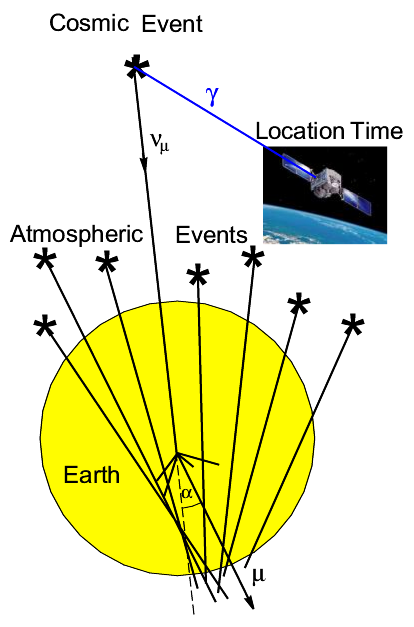
\includegraphics[keepaspectratio,height=15cm]{atm-bkg}
\end{center}

\newpage

\begin{itemize}
\item No signal $\rightarrow$ Give flux upper limit
\item Link observations and flux via Effective area
\item[] $ A_{eff} \equiv$ obs. event rate~/~incoming flux
\item[] $\rightarrow$ Flux limit = max. event rate~/~$A_{eff}$
\end{itemize}
%
\begin{center}
{\blue $\nu_{\mu}+\bar{\nu}_{\mu}$ Effective area (solid angle averaged)}\\
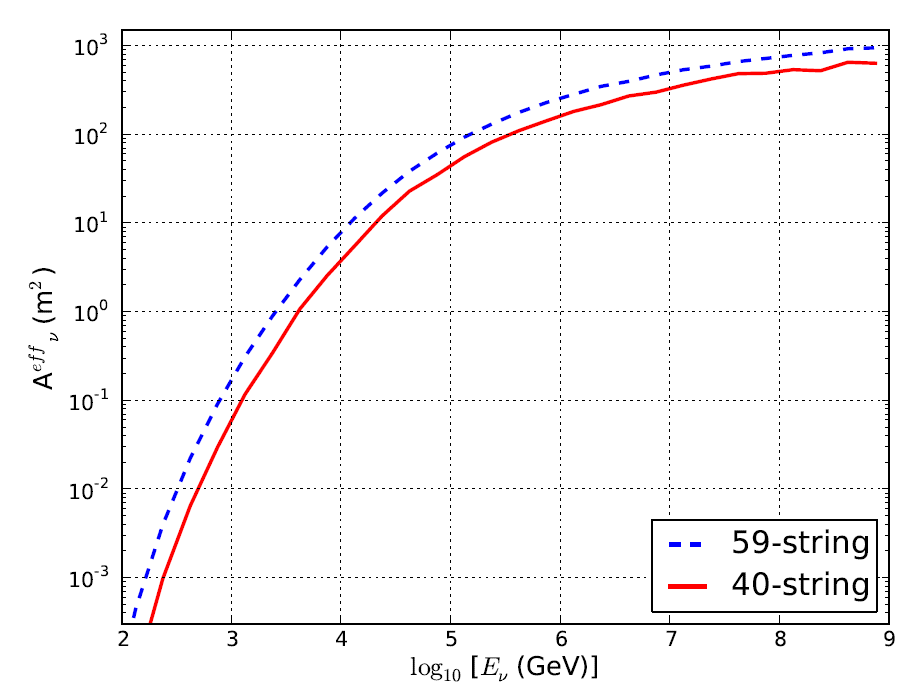
\includegraphics[keepaspectratio,height=9.5cm]{ic59+40-eff-area}
\end{center}

\Tr
\onecolumn
\begin{center}
{\blue IceCube limit (Nature 484 (2012) 351)}\\
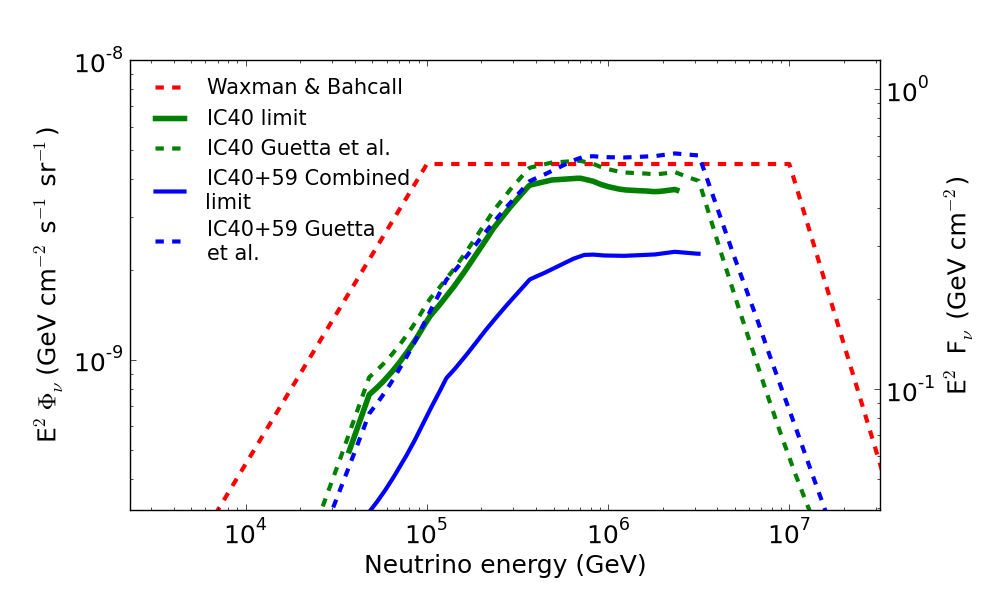
\includegraphics[keepaspectratio,height=11cm]{ic59+40-grb-limit2}
\end{center}
%
\begin{itemize}
\item GRBs are not (the only) UHECR sources $\rightarrow$ AGN ?
\item[] {\blue Or :} Efficiency of $\nu$ production lower than expected
\item Models with standard parameters excluded by observations
\end{itemize}
